% !TEX root = main.tex
% Tipo di documento. L'uso di twoside implica che i capitoli inizino sempre con la prima pagina a sinistra, eventualmente lasciando una pagina vuota nel capitolo precedente. Se questa cosa è fastidiosa, è possibile rimuoverlo. 
\documentclass[a4paper, twoside,openright]{report}
% \documentclass[a4paper,openright]{report}

% \usepackage{fancyhdr}
% \pagestyle{fancy}
% \fancyhf{}
% \lhead{\rightmark}
% \rhead{\textbf{\thepage}}
% % \fancyfoot{}
% \setlength{\headheight}{12.5pt}
% Rimuove il numero di pagina all'inizio dei capitoli
% \fancypagestyle{plain}{
%   \fancyfoot{}
%   \fancyhead{}
%   \renewcommand{\headrulewidth}{0pt}
% }


\usepackage{graphicx} % Required for inserting images
\setkeys{Gin}{width=0.6\columnwidth}

\usepackage[utf8]{inputenc}

\usepackage{hyperref}
\usepackage{adjustbox}

\usepackage{wrapfig}

\usepackage{enumitem}
\renewcommand{\labelitemi}{$\diamond$}
\renewcommand{\labelitemiii}{$\circ$}
\setlist[enumerate,2]{label=\roman*.}
\setlist[enumerate,3]{label=(\alph*)}

\setitemize{noitemsep}
\setenumerate{noitemsep}
\setlist{noitemsep}

\usepackage{paracol}
\usepackage{multicol}
\usepackage{booktabs}


\usepackage{geometry}

\usepackage{color}

\usepackage{listings}
% \usepackage{minted}

\usepackage{amsmath}
\usepackage{amssymb}
\usepackage{amsfonts}
\usepackage{mathtools}
\usepackage{bm}
\usepackage{nicefrac, xfrac}

\usepackage{wasysym}

% Uso dei colori
\usepackage[dvipsnames,table,xcdraw]{xcolor}
\usepackage{colortbl}
\usepackage{rotating}
\usepackage{adjustbox}

\usepackage{multirow}
\usepackage{booktabs}
\usepackage{makecell}


\usepackage{tikz}
\usetikzlibrary{automata, arrows,bending}
\usetikzlibrary{positioning}
\usetikzlibrary{shapes.geometric}
\usepackage{parskip}
\usepackage{changepage}

\usepackage{soul}
\usepackage{cancel}

% This are needed because the correct double quotes would be ``'' or ``",
% but i've always written "text"
% TODO - check whether this affects listing environment
% \usepackage [english]{babel}
% \usepackage [autostyle, english = american]{csquotes}
% \MakeOuterQuote{"}

\geometry{margin=0.6in}

\setlist[description]{itemsep=0em,topsep=0.5em,parsep=0em}
\setlist[itemize]{itemsep=0em,topsep=0pt}
\setlist[enumerate]{itemsep=0em,topsep=0pt}

\hypersetup{
    colorlinks=true,
    linkcolor=black,
    filecolor=mauve,
    urlcolor=blue,
}

\definecolor{gray}{gray}{0.3}
\definecolor{verylightgray}{gray}{0.95}
\definecolor{blue}{rgb}{0,0,1}
\definecolor{mauve}{rgb}{0.58,0,0.82}
\definecolor{darkred}{rgb}{0.3,0,0}
\definecolor{darkgreen}{rgb}{0,0.3,0}
\definecolor{darkgray}{gray}{0.15}



\newenvironment{notes}{
\par
\color{gray}
\small}

\newcommand{\note}[1]{\begin{notes}{#1}\end{notes}}
\newcommand{\nl}[0]{\parskip = \baselineskip}
\newcommand{\lst}[1]{\lstinline{#1}}
\newcommand{\ra}{\xrightarrow{\hspace*{2em}}}
\newcommand{\ns}{\setlength{\parskip}{0em}}

\newlength{\currentparindent}
\newcommand{\labelitemize}[2]{
\setlength{\currentparindent}{\parindent}
\setlength{\parindent}{0pt}

\begin{minipage}{0em} % Adjust the width as needed
    \makebox[0em][c]{\rotatebox{90}{\small #1}}
\end{minipage}
\begin{minipage}{\dimexpr\columnwidth-1cm\relax}
    #2
\end{minipage}
\setlength{\parindent}{\currentparindent}
}
\newcommand{\colfill}{\vspace{\fill}}

\newcommand{\framed}[1]{
\begin{center}
\fbox{
    \begin{minipage}{0.8\columnwidth}
        #1
    \end{minipage}
}
\end{center}}

\newcommand{\framedt}[2]{
\begin{center}
\fbox{
    \begin{minipage}{0.8\columnwidth}
        \vspace*{1em}
        \begin{center}
            \textbf{\ul{#1}}
        \end{center}
        \nl
        #2
    \end{minipage}
}
\end{center}}

\newcommand{\proscons}[4]{
    \begin{paracol}{2}
        \labelitemize{\color{darkgreen}\ul{\textit{#1}}}{
           \color{darkgreen}
           #3
        }
        \switchcolumn
        \labelitemize{\color{darkred}\ul{\textit{#2}}}{
           \color{darkred}
           #4
        }
     \end{paracol}
}

\newcommand\hcancel[2][black]{\setbox0=\hbox{$#2$}%
\rlap{\raisebox{.45\ht0}{\textcolor{#1}{\rule{\wd0}{1pt}}}}#2} 


\lstset{frame=false,
 showstringspaces=false,
 breaklines=true;
 columns=flexible,
 basicstyle={\small\ttfamily},
 keywordstyle=\color{blue},
 commentstyle=\color{darkgreen},
 stringstyle=\color{mauve}
 tabsize=3
}

\newtheorem{definition}{Definition}[chapter]
\newtheorem{theorem}{Theorem}[chapter]

\usepackage{fancyhdr}
% \usepackage{nameref,autoref}

\pagestyle{fancy}
\fancyhf{}
\fancyhead[LE,RO]{\thepage} % Page number on Outer side of header on each page
\fancyhead[LO]{\leftmark} % section title on Left side of header on Odd pages
\fancyhead[RE]{\rightmark} % subection title on Right side of header on Even pages
\fancyfoot{}
\renewcommand{\headrulewidth}{0.4pt} % Width of line under the header
% \setcounter{secnumdepth}{2} % Depth of sectioning commands to include in the table of contents

% Rimuove il numero di pagina all'inizio dei capitoli
\fancypagestyle{plain}{
  \fancyfoot{}
  \fancyhead{}
  \renewcommand{\headrulewidth}{0pt}
}

\usepackage{emptypage}



\title{Data Mining - Appunti}
\author{Francesco Lorenzoni}
\date{Febrero 2025}


\makeatletter
\renewcommand{\l@section}{\@dottedtocline{1}{1.5em}{2.6em}}
\renewcommand{\l@subsection}{\@dottedtocline{2}{2.5em}{3.6em}}
\renewcommand{\l@subsubsection}{\@dottedtocline{3}{3.5em}{4.5em}}
\makeatother
\mtcsettitle{parttoc}{Contents of this Part} % Set the title for the part TOC


\begin{document}
\doparttoc[n]

\maketitle
\tableofcontents

\part{Introduction to Data Mining}
\parttoc
\chapter{Práctica 4 y 5}

% No necesario con minted (se especifica al usar el entorno)
\lstset{language=python}

% Preface
% \note{Soy un estudiante italiano en Erasmus. Hablo español bastante bien, pero me resulta más natural escribir en inglés; sin embargo, decidí escribir en español para practicar, con la ayuda de algunos traductores cuando era necesario. Si hay algo mal escrito o poco claro, estoy a disposición para cualquier aclaración.}

\section{Ejercicios 1/2/3 - \texttt{sin\_vocales}}

\subsection{Ejercicio 1 - Función inicial}
\begin{lstlisting}[captionpos=b,caption={Función inicial}]
   def sin_vocales (s):
      """
      devuelve el argumento s sin vocales
      """
      vocales = 'aeiou'
      s_sinVocales = ' '
      for ch in s:
         pos = vocales.find(ch)
         if pos == -1: #ch no es vocal
            s_sinVocales = s_sinVocales + ch
      return s_sinVocales
\end{lstlisting}

Esta es la función inicial que se nos ha dado, y que parece funcionar, pero solo con pruebas demasiado sencillas.

\subsection{Ejercicio 2 - Prueba de la función}

Abajo en el código \ref{code:pruebas}, después de la discusión de los dos errores encontrados, hay la función	de prueba completa \lstinline{test_sin_vocales()} que comprueba la función \lstinline{sin_vocales(s)}. 


\begin{paracol}{2}
   \colfill
   El primero error en la función dada \lstinline{sin_vocales(s)} es que \ul{no se tiene cuenta de las \textbf{mayúsculas} y \textbf{minúsculas}}. Por lo tanto, la función no elimina las vocales mayúsculas. Para solucionarlo, es suficiente añadir a la lista de vocales la versión mayúscula de cada vocal.
   \colfill

   \switchcolumn

   \begin{lstlisting}
def test_sin_vocales():
   s = "el agua esta mojada"
   exp = "l g st mjd"
   assert sin_vocales(s) == exp

   ...
      
   s = "El AgUe eStA mOjAdA"
   exp = "l g St mjd"
   assert sin_vocales(s) == exp
   \end{lstlisting}
\end{paracol}

\begin{lstlisting}[captionpos=b,caption={\lstinline|sin_vocales()| con vocales mayúsculas}, label={code:sin_vocales1}]
   def sin_vocales (s:str):
      vocales = 'aeiouAEIOU'
      s_sinVocales = ''
      for ch in s:
         pos = vocales.find(ch)
         if pos == -1: #ch no es vocal
            s_sinVocales = s_sinVocales + ch
      return s_sinVocales
\end{lstlisting}

\newpage
\begin{paracol}{2}
   \colfill
   El segundo error es que la función \ul{no tiene cuenta de los \textbf{acentos}}. Por lo tanto, la función no elimina las vocales acentuadas.
   \begin{lstlisting}
   assert sin_vocales("áÉíÓú") == "" # falla
   \end{lstlisting}
   Para solucionarlo, es suficiente añadir a la lista de vocales la versión acentuada de cada vocal.

   \begin{lstlisting}
   vocales = 'aeiouAEIOUáéíóúàèìòùäëïöüâê
   îôûÁÉÍÓÚÀÈÌÒÙÄËÏÖÜÂÊÎÔÛãõÃÕ'
   \end{lstlisting}

   Esta solución no parece muy elegante, ya que la lista de vocales se vuelve muy larga. Buscando sobre el internet he visto que una solución más elegante sería usar una expresión regular para eliminar todas las vocales, acentuadas o no. Para ello, se puede usar el módulo \lstinline{re} de Python, junto con \lstinline{unicodedata}, como se muestra en el código a la derecha.
   \colfill

   \switchcolumn
   \colfill
   \begin{lstlisting}[label={code:unicodedata},captionpos=b,caption={Código para eliminar vocales y diacríticos que utiliza \lstinline{unicodedata}}]
import unicodedata
import re

def sin_vocales(s):
   # Normaliza el texto separando los caracteres básicos de sus diacríticos
   s_norm = unicodedata.normalize('NFD', s)
   # Elimina todas las vocales base y los diacríticos
   s_sin_vocales = re.sub(r'[aeiouAEIOU\u0300-\u036f]', '', s_norm)
   return s_sin_vocales
   \end{lstlisting}
   \colfill
\end{paracol}

\vspace{2em}

\begin{lstlisting}[captionpos=b,caption={Pruebas que he escrito}, label={code:pruebas}]
def test_sin_vocales():
   s = "el agua esta mojada"
   exp = "l g st mjd"
   assert sin_vocales(s) == exp
   s = "aieou"
   exp = ""
   assert sin_vocales(s) == exp
   s = "123greee"
   exp = "123gr"
   assert sin_vocales(s) == exp
   s = "El AgUe eStA mOjAdA"
   exp = "l g St mjd"
   assert sin_vocales(s) == exp
   s = "àéíóú"
   exp = ""
   assert sin_vocales(s) == exp
   s = "are you ok?"
   exp = "r y k?"
   assert sin_vocales(s) == exp
   s = ""
   exp = ""
   assert sin_vocales(s) == exp
   s = "A"
   exp = ""
   assert sin_vocales(s) == exp
   
\end{lstlisting}
\subsection{Ejercicio 3/4 - Corregir la función y añadir pruebas}

\begin{lstlisting}[captionpos=b,caption={\lstinline|sin_vocales()| corregida}, label={code:sin_vocales}]
   def sin_vocales (s:str):
      vocales = 'aeiouAEIOUáéíóúàèìòùäëïöüâêîôûÁÉÍÓÚÀÈÌÒÙÄËÏÖÜÂÊÎÔÛãõÃÕ'
      s_sinVocales = ''
      for ch in s:
         pos = vocales.find(ch)
         if pos == -1: #ch no es vocal
            s_sinVocales = s_sinVocales + ch
      return s_sinVocales
\end{lstlisting}

Para evitar el uso del paquete adicional \lstinline{unicodedata}, he preferido utilizar simplemente listas de vocales que incluyen también las vocales acentuadas.

He añadido al fichero \texttt{.py} la función que nos ha dado en el ejercicio, per controllare che anche quei test passassero.

\newpage
\section{Ejercicio 5 - \texttt{cantidad\_numeros}}
\begin{lstlisting}[captionpos=b,caption={Solución sencilla}]
def cantidad_numeros_sencilla(s: str):
   """
   Esta función recibe una cadena de texto y devuelve la cantidad de números que contiene.
   N.B. números, no digitos!
   """
   return len(re.findall(r'\d+', s))
\end{lstlisting}

Esta primera solución funciona y es concisa, pero no tiene en cuenta los números decimales (como $12.34$) y las notaciones científicas (como $12\cdot 10^6$ o $10^{-2}$). 
Para solucionarlo, es necesario modificar la expresión regular para que también considere estos casos.

\begin{lstlisting}[captionpos=b,caption={Solución que incluye números decimales y notaciones científicas}]
      
def cantidad_numeros(s: str):
   """
   Esta función recibe una cadena de texto y devuelve la cantidad de números que contiene.
   
   Números decimales (como 12.34) y notaciones científicas (como 12*10^6 o 10^(-2)) son considerados números.
   """
   # Identificar números decimales (como 12.34)
   decimal_pattern = r'-?\d+\.\d+'
   decimal_matches = re.findall(decimal_pattern, s)
   
   # Eliminar los números decimales ya encontrados para evitar contar dos veces
   for match in decimal_matches:
       s = s.replace(match, ' ', 1)
   
   # Identificar notaciones científicas (como 12*10^6 o 10^(-2))
   scientific_pattern = r'\d+\*10\^\(?\-?\d+\)?'
   scientific_matches = re.findall(scientific_pattern, s)
   
   # Eliminar las notaciones científicas de la cadena
   for match in scientific_matches:
       s = s.replace(match, ' ', 1)
   
   # Encontrar los números restantes (enteros)
   # Modificamos el patrón para capturar secuencias de dígitos en cualquier contexto
   remaining_pattern = r'\d+'
   remaining_matches = re.findall(remaining_pattern, s)
   
   # Contar el total de números encontrados
   return len(decimal_matches) + len(scientific_matches) + len(remaining_matches)
\end{lstlisting}

\newpage
\begin{paracol}{2}
   
   \begin{lstlisting}[captionpos=b,caption={Mis pruebas para \lstinline|cantidad_numeros()|}, label={code:cantidad_numeros}]
def test_cantidad_numeros():
   s = "12 356 53333"
   assert cantidad_numeros(s) == 3
   s = "asfa432asf23"
   assert cantidad_numeros(s) == 2
   s = ""
   assert cantidad_numeros(s) == 0
   s = "1"
   assert cantidad_numeros(s) == 1
   s = "fwgds"
   assert cantidad_numeros(s) == 0
   s = "1 fhsdSGG 4"
   assert cantidad_numeros(s) == 2
   s = "-12 + 34 -12-133 "
   assert cantidad_numeros(s) == 4
   s = "12.34 56.78"
   assert cantidad_numeros(s) == 2
   s = "12*10^6"
   assert cantidad_numeros(s) == 1
   s = "23*10^(-2)"
   assert cantidad_numeros(s) == 1
   s = "23*10^(64) + 12.34"
   assert cantidad_numeros(s) == 2
   s = "asgre23*10^(-2)asfg10^2"
   assert cantidad_numeros(s) == 2
   s = "asgre23*10^(-2)asfg10^2agr12.34"
   assert cantidad_numeros(s) == 3
   \end{lstlisting}

   \switchcolumn

   \begin{lstlisting}[captionpos=b,caption={Pruebas ordenadas como estan en el documiento}, label={code:cantidad_numeros2}]
def test_cantidad_numeros_doc():
   # Varios números en la cadena
   s = "un 1, un 201 y 2 unos"   
   assert cantidad_numeros(s) == 3
   # Sin números en la cadena
   s = "sin numeros"   
   assert cantidad_numeros(s) == 0
   # Un solo número en la cadena
   s = "2345543"    
   assert cantidad_numeros(s) == 1
   # Diferentes longitudes de números
   s = "1 22 333 4444 55555"    
   assert cantidad_numeros(s) == 5
   # Números separados por espacios
   s = "123 456 789"    
   assert cantidad_numeros(s) == 3
   # Números separados por comas
   s = "12,34,56,78"    
   assert cantidad_numeros(s) == 4
   # Números rodeados de texto
   s = "numero123numero456numero"   
   assert cantidad_numeros(s) == 2
   # Una cadena continua de números
   s = "123456789"   
   assert cantidad_numeros(s) == 1
   # Números al inicio y al final
   s = "1 starting and ending 2"    
   assert cantidad_numeros(s) == 2
   # Número al final 
   s = "ending with number 5"   
   assert cantidad_numeros(s) == 1
   # Números en una cadena simple
   s = "3 6 9"   
   assert cantidad_numeros(s) == 3
   # Sin números en la cadena
   s = "sinnumeros"    
   assert cantidad_numeros(s) == 0
   # Números mezclados con texto
   s = "123unnumero456"   
   assert cantidad_numeros(s) == 2
   # Números negativos
   s = "-5 10 -15"  
   assert cantidad_numeros(s) == 3
   \end{lstlisting}
\end{paracol}

\newpage
\section{Ejercicio 6 - \texttt{sin\_vocales} con prueba parametrizada}

\begin{lstlisting}
@pytest.mark.parametrize ("entrada , salida_esperada " ,[
   ("El agua esta mojada", "l g st mjd"),
   ("mojada bañando en el agua", "mjd bñnd n l g"),
   ("ahora termina bien", "hr trmn bn"),
   ("", ""),
   ("a", ""),
   ("m", "m"),
   ("unstringsinespacios", "nstrngsnspcs"),
   ("MAYUSculas FUNCIOnaN", "MYScls FNCnN"),
   ("krt yhgf dwpq", "krt yhgf dwpq"),
   ("aeoiuuuoiea", ""),
   ("disco de los 80", "dsc d ls 80"),
   ("signos como ? y ! y ¡", "sgns cm ? y ! y ¡"),
   ("ábc élla ó", "bc ll "),
   ("Óm tambien mayÚsculÁs", "m tmbn myscls")
   ])

def test_sin_vocales_parametrizado(entrada, salida_esperada):
   """
   testea la función sin_vocales
   """
   assert sin_vocales (entrada) == salida_esperada
\end{lstlisting}

Esta es una forma alternativa de escribir los test, que permite de parametrizar la función driver de test.

En comparación con el test set anterior del pdf, hemos añadido pruebas que incluyen vocales con acento. La función \lstinline|sin_vocales| no va a cambiar porque ya había tenido en cuenta los acentos en el ejercicio anterior.




\chapter{Tarea 2}

% TAREA 2.

%     Visualiza el siguiente vídeo:

% https://www.google.com/search?client=firefox-b-d&q=Kaspersky+Industrial+CyberSecurity+demonstration+for+Energy+sector+-+Bing+video+#fpstate=ive&vld=cid:fc74c561,vid:7LNtjWx17mA,st:0


\framedt{Tarea a realizar}{

   Visualiza el siguiente vídeo:
   \href{
      https://www.youtube.com/watch?v=7LNtjWx17mA
   }{youtube.com/watch?v=7LNtjWx17mA}
   
   \begin{itemize}
   	\item Identifica en la red industrial los componentes físicos, ciberfísicos, y ciber
	\item Identifica los tipos de ataque que se describen en el vídeo, y explica brevemente como piensas que se podrían implementar.
	\item Explica cómo plantea la solución de Kaspersky en el vídeo la defensa frente a los posibles ataques.
   \end{itemize}
}


%     Contesta a las siguientes preguntas:

%     Identifica en la red industrial que se describe en el vídeo:

% a. Lo componentes físicos

% b. Los componentes ciberfísicos

% c. Los componentes ciber

%     Identifica los tipos de ataque que se describen en el vídeo, y explica brevemente como piensas que se podrían implementar.

%     Explica cómo plantea la solución de Kaspersky en el vídeo la defensa frente a los posibles ataques.

\begin{figure}[htbp]
   \centering
   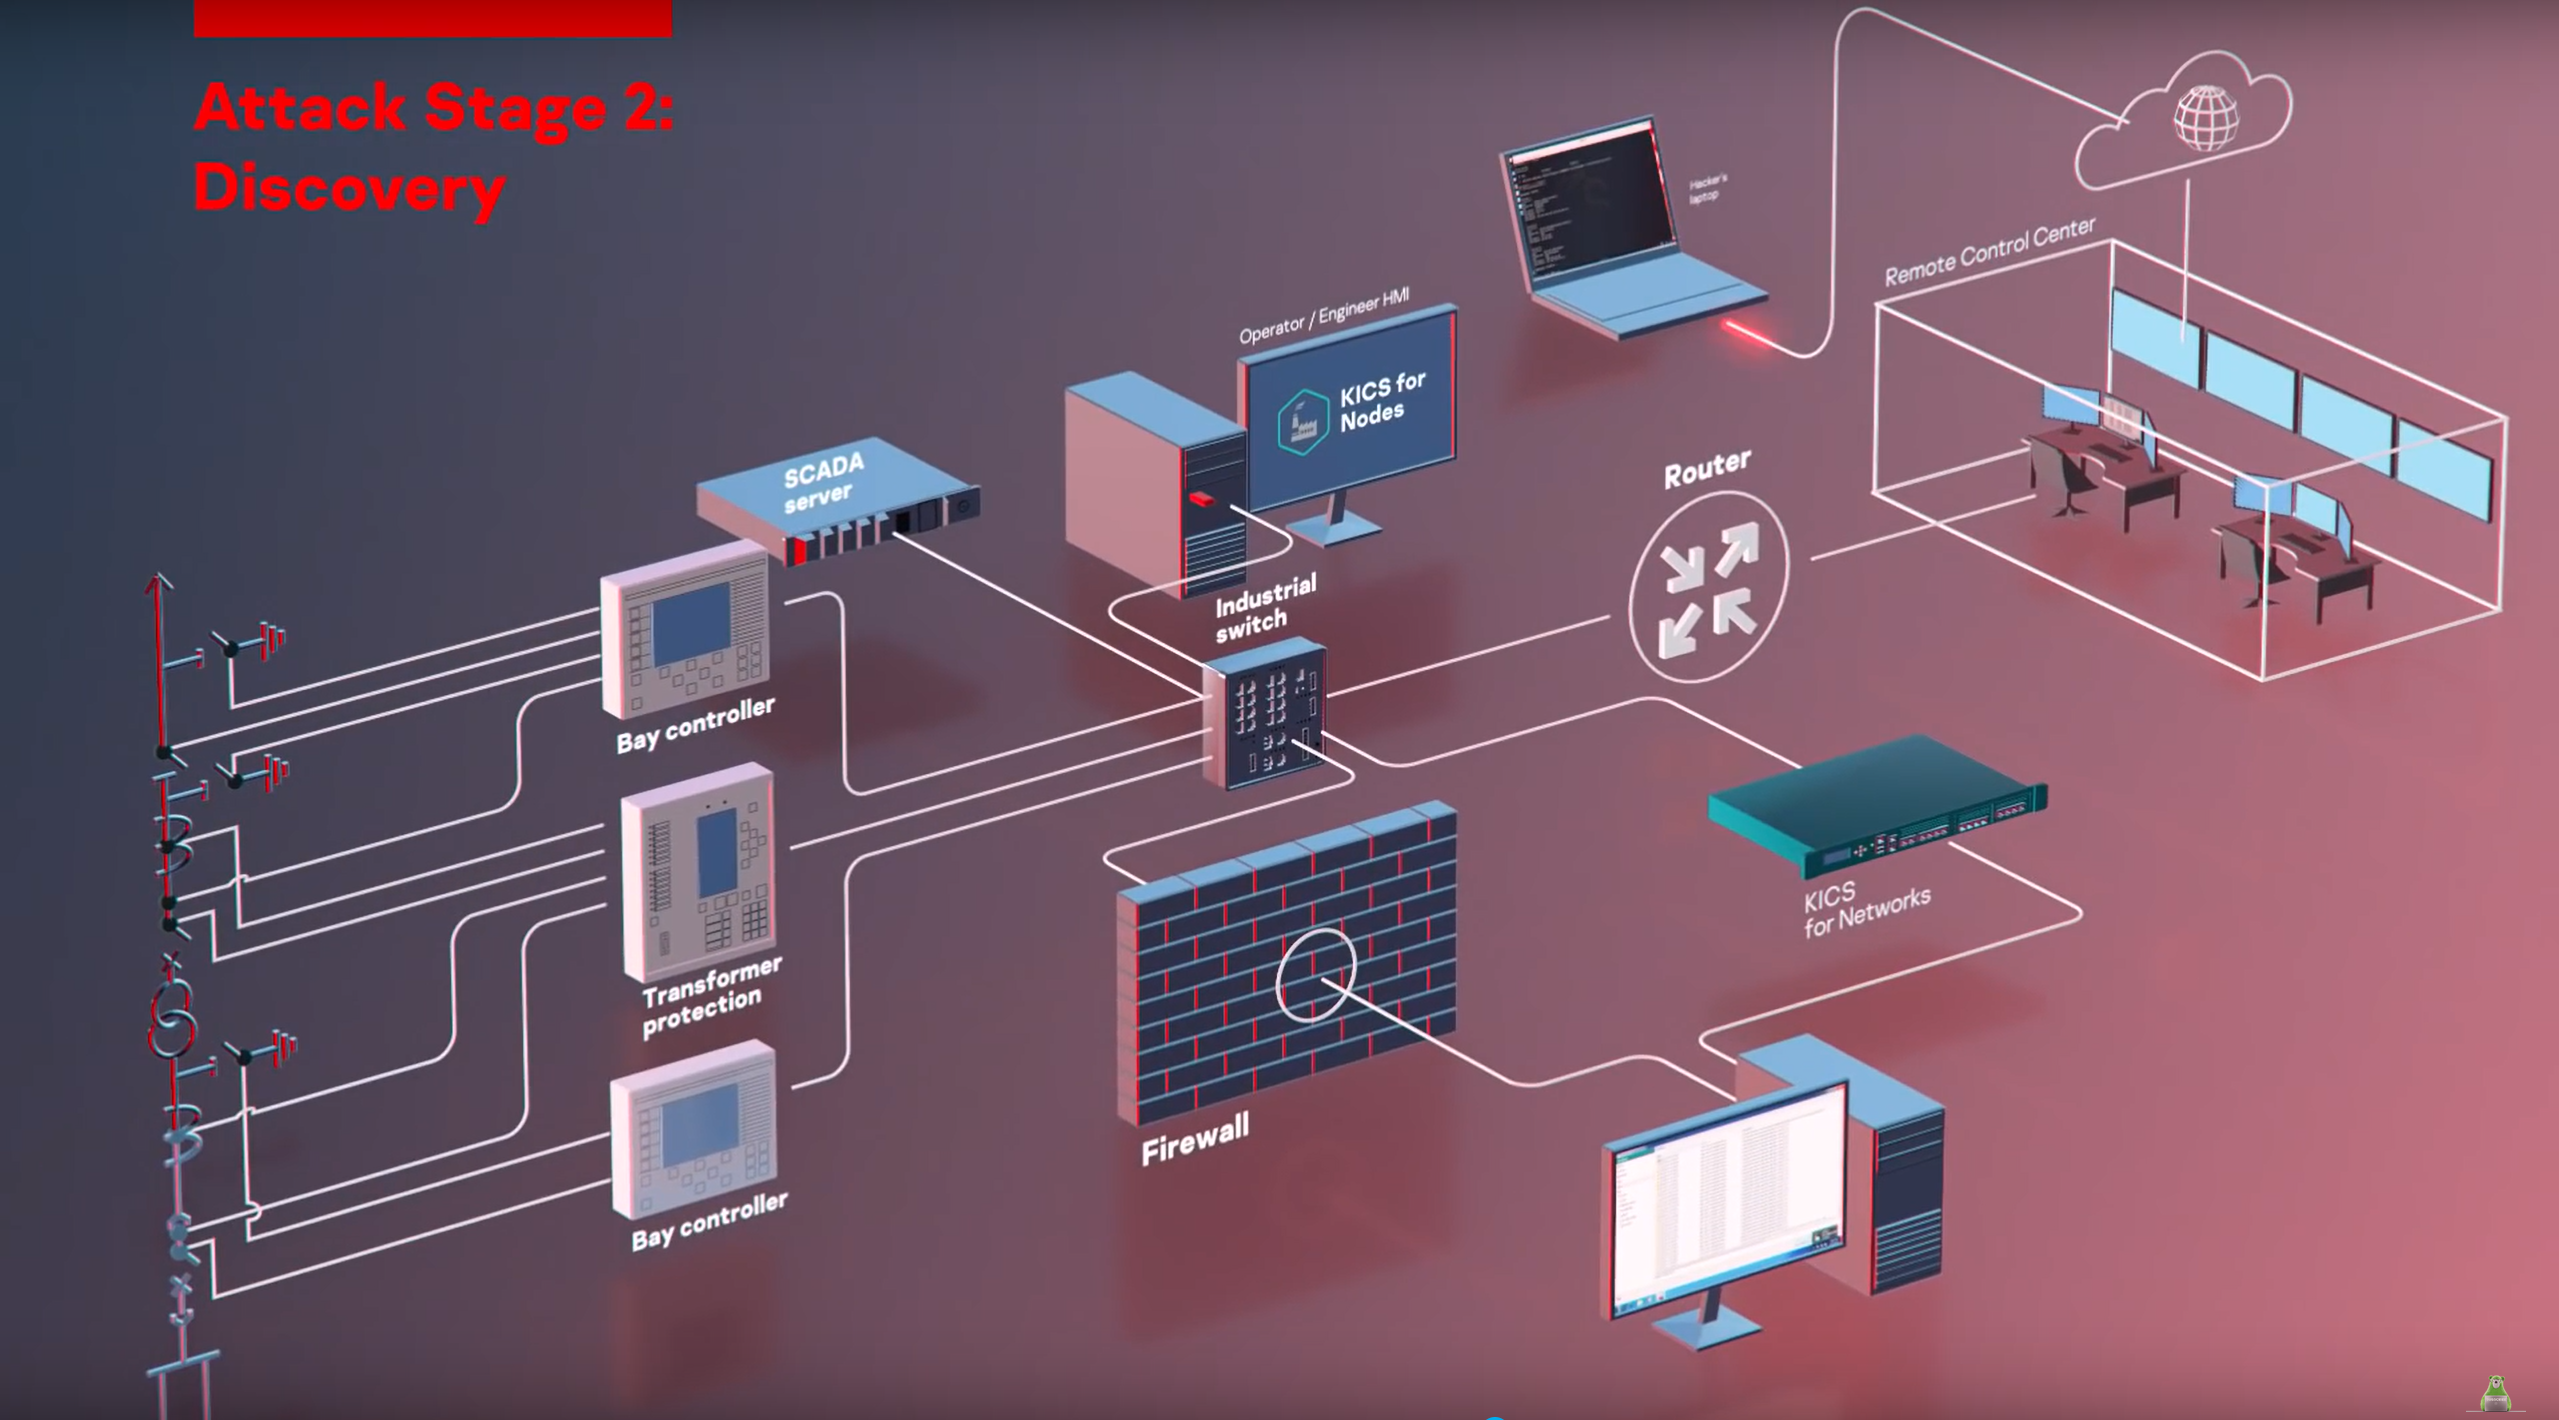
\includegraphics{images/ICSscenario.png}
   \caption{Escenario representado en el vídeo}
   \label{fig:ICSscenario}
\end{figure}


\section{Componentes de la red industrial}

\begin{itemize}
   \item \textbf{Componentes físicos:}
   \begin{itemize}
      \item 100kv high-voltage incoming line
      \item Power transformer
      \item 10kV bus feeder
      \item Primary switching equipment
   \end{itemize}
   \item \textbf{Componentes ciberfísicos:}
   \begin{itemize}
      \item transformer protection
      \item 2 bay controllers
      \item Industrial Ethernet switch
   \end{itemize}
   \item \textbf{Componentes ciber:}
   \begin{itemize}
      \item Kaspersky Industrial CyberSecurity
      \begin{itemize}
         \item \textsc{KICS} for Nodes - Endpoint Protection
         \item \textsc{KICS} for Network - Anomaly and Breach Protection
         \item Centralized security management
         \item Kasperky Security Center - Manager installed on nodes
      \end{itemize}
      \item Router
      \item Firewall
      \item Remote Control Center tools
      \item SCADA server
   \end{itemize}
\end{itemize}

\subsection{Kaspersky Industrial CyberSecurity (\textsc{KICS})}
% Software / hardware / virtual appliance
\begin{paracol}{2}
   
   Las ---``claimed''--- features de \textsc{KICS} son las siguientes:
   \begin{itemize}
	\item Passive traffic analysis
	\item No influence on network stability
	\item Detection of:
	\begin{itemize}
      \item Unauthorized network access
      \item Cyberattacks and intrusions
      \item Unauthorized commands to industrial equipment
      \item Technological parameters anomalies:
      \begin{itemize}
         \item Rules based
	      \item Machine learning
      \end{itemize}
      \item Assets and its parameters
      \item Abnormal dataflow on network map
   \end{itemize}
\end{itemize}

\switchcolumn

\colfill
\begin{figure}[htbp]
   \centering
   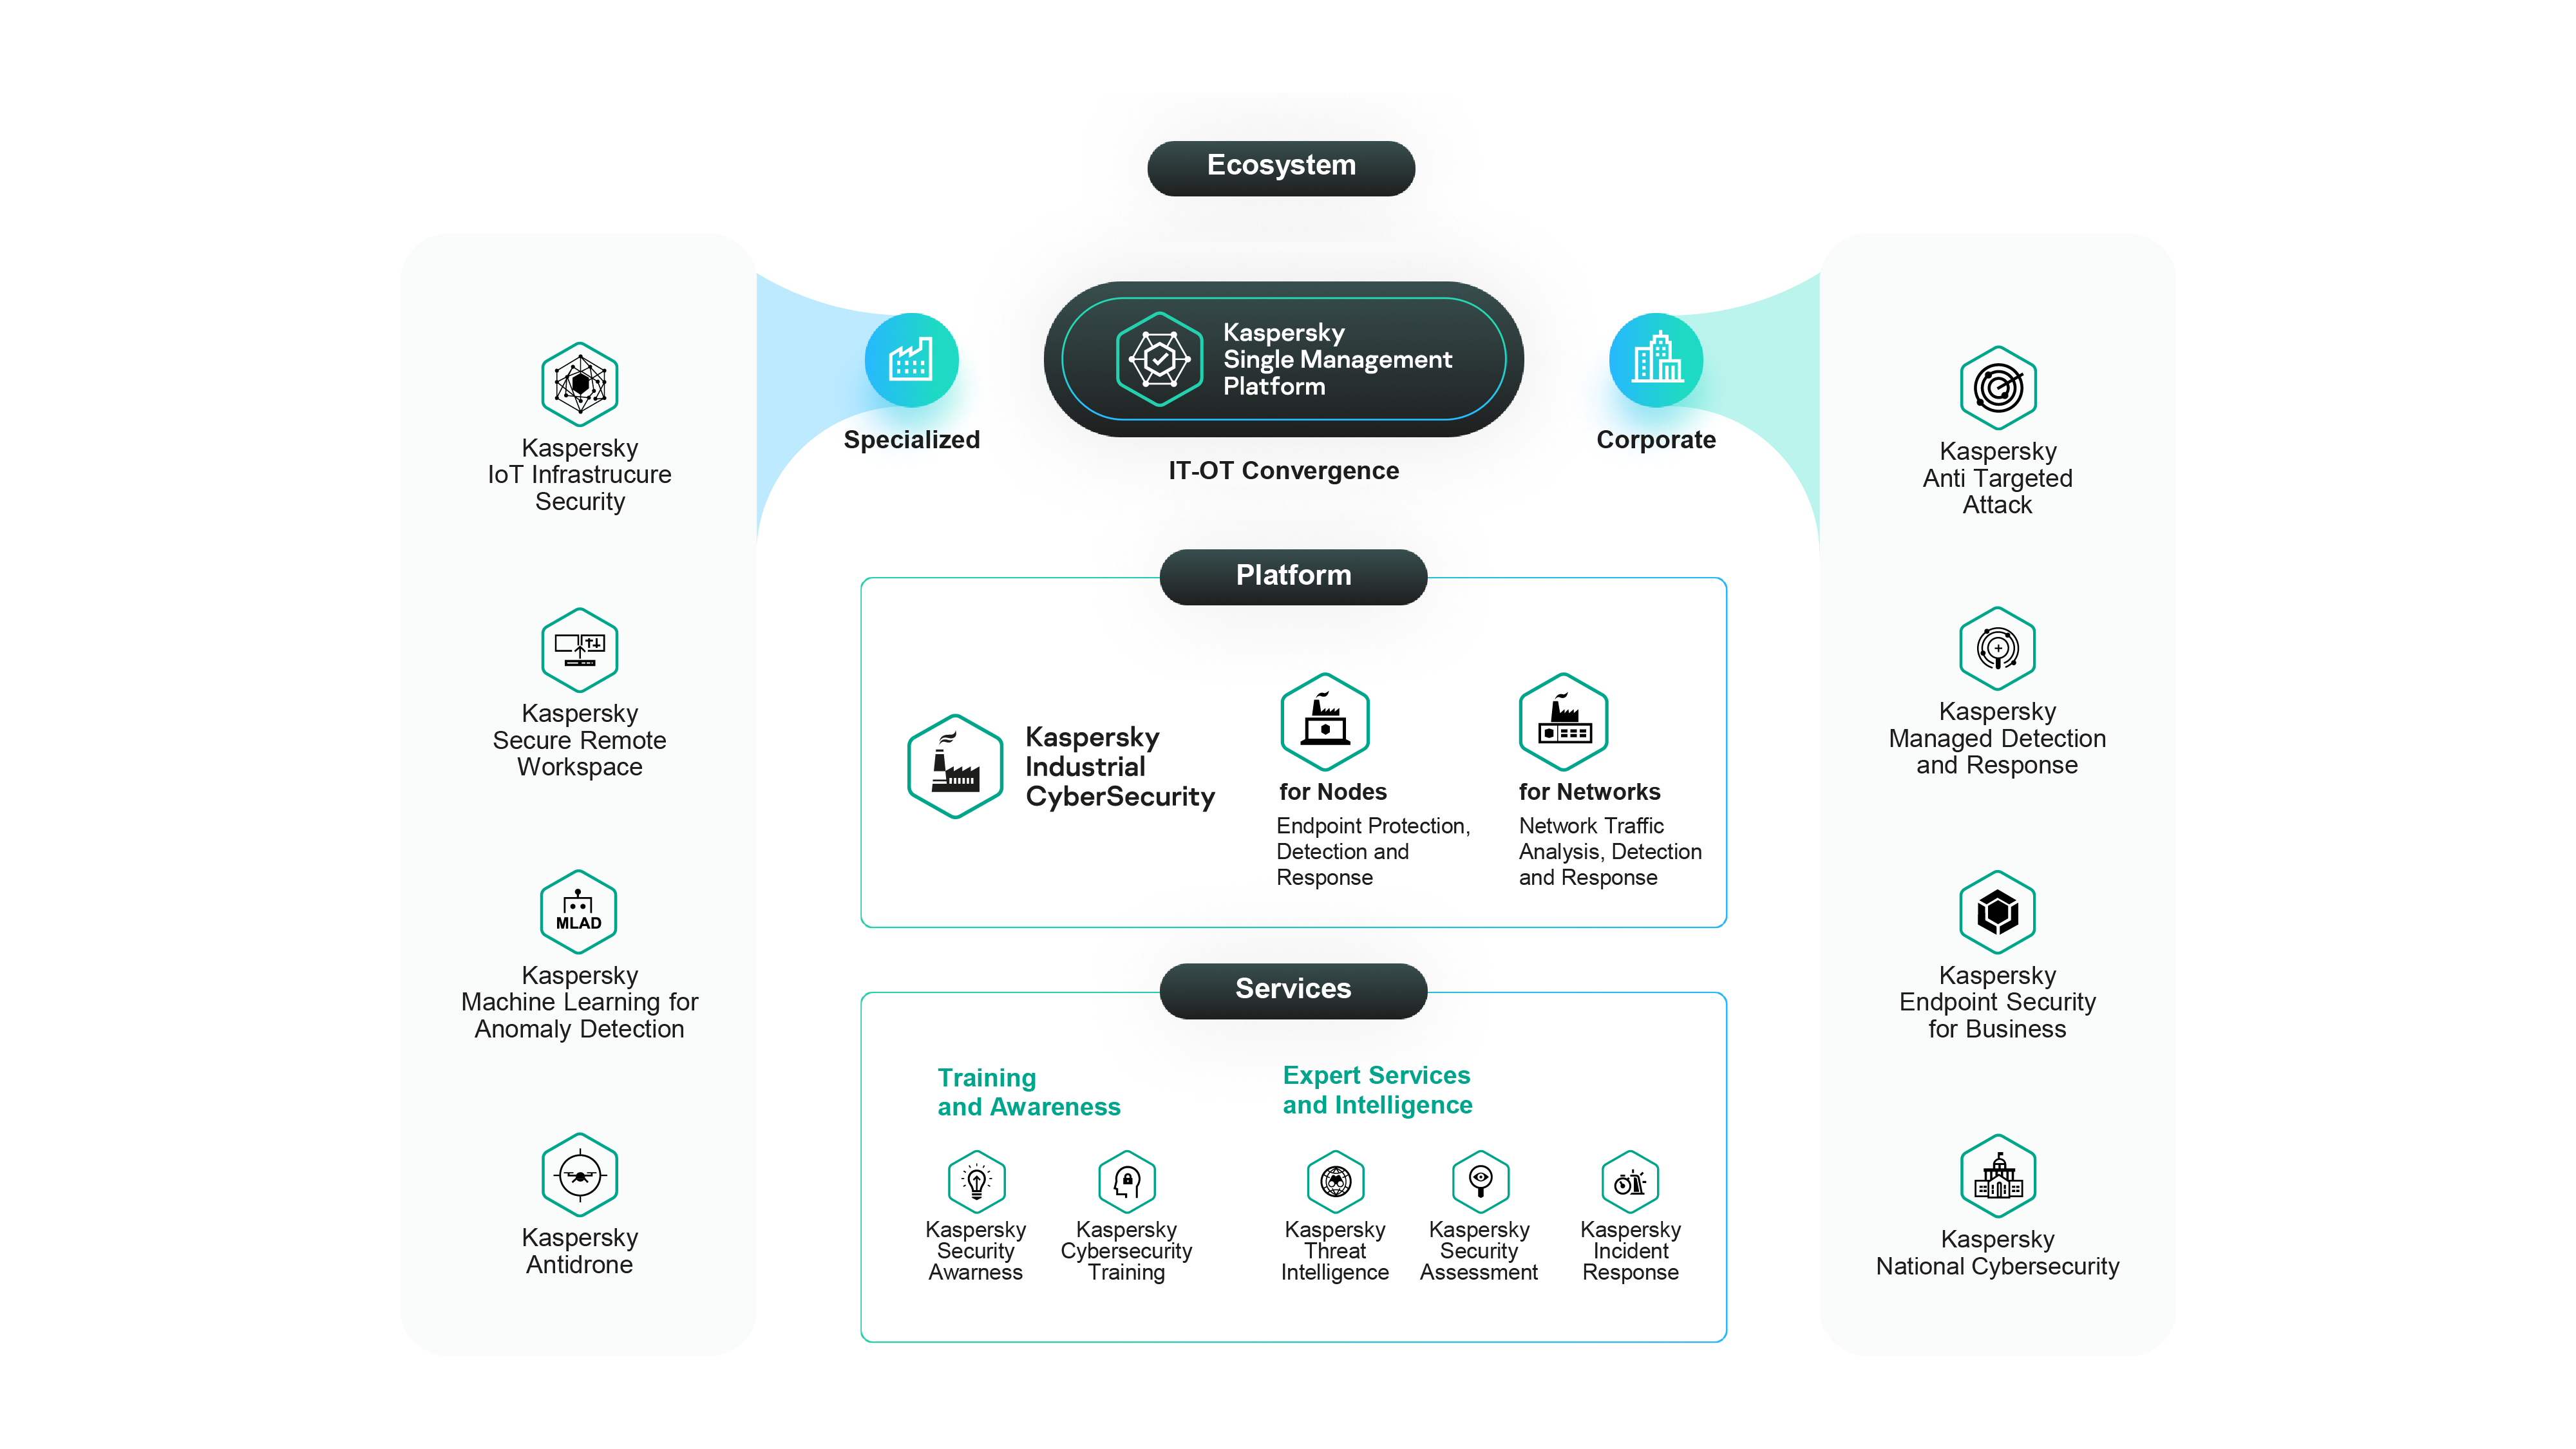
\includegraphics[width=0.95\columnwidth]{images/KICS.png}
   \caption{\textsc{KICS} schema}
   \label{fig:KICS}
\end{figure}
\colfill

\end{paracol}
\section{Ataque sobre la infraestructura industrial y defensa}

El ataque que se muestra en el video comprende tres fases, también se analizan las posibles implementaciones de cada una de ellas:
\begin{enumerate}
   \item \textbf{Breach} - \textit{Obtener acceso a un componente}
   \begin{itemize}
      \item Instalar un malware a traves de un documiento \texttt{.pdf} en un \textsc{usb}, que cuando se abre, se conecta al atacante, que obtiene acceso la computadora infectada, que puede utilizar como fuente para futuros ataques en la red.
      \item \textit{\ul{Defensa}} - \textsc{KICS} for Networks detecta una comunicación no autorizada entre la computadora infectada y una dirección IP externa y un payload potencialmente peligroso, y envía una alerta a \textit{Kaspersky Security Center}.
      \note{Si puede bloquear el ataque aquí, pero en el video se supone que no lo haces para mostrar el comportamiento defensivo en las fases siguientes}
      \begin{figure}[htbp]
         \centering
         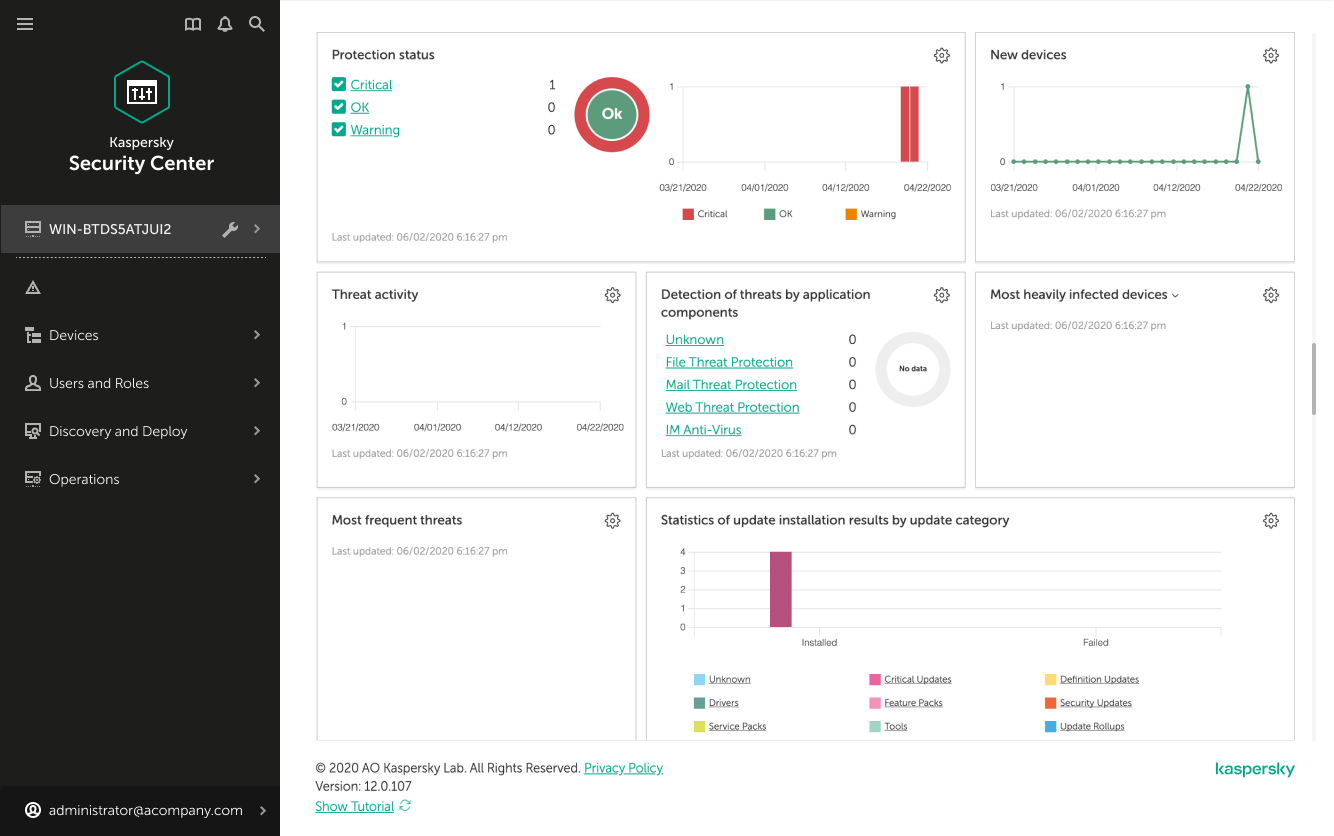
\includegraphics{images/KasperskySC.png}
         \caption{Kaspersky Security Center}
         \label{fig:KasperskySC}
      \end{figure}
   \end{itemize}
   \item \textbf{Discovery} - \textit{Obtener información y datos sobre el sistema}
   \begin{itemize}
      \item A través del componente infectado, el atacante puede \textbf{escanear} la red y obtener información sobre los dispositivos ciber y ciberfísicos conectados, lo que le permite establecer las vulnerabilidades actuales y planificar futuros ataques explotándolas.
      A menudo las comunicaciones entre dispositivos ciberfísicos y ciber carecen de \textbf{encriptación}, potencialmente exponiendo datos y credenciales sensibles.\\
      Si no hay suficiente segmentación de red, o si falta apropiada configuración de los Firewalls, este proceso puede ser aún más facilitado.
      \item \textit{\ul{Defensa}} - \textsc{KICS} for Networks detecta un escaneo de red no autorizado y envía una alerta a Kaspersky Security Center. Imagino que \textsc{KICS} también puede detectar cualquier movimiento lateral del atacante.
   \end{itemize}
   \item \textbf{Technlogical Attack} - \textit{Ataque a la infraestructura}
   \begin{itemize}
      \item Si no se bloquea el ataque en la fase anterior, el atacante puede enviar \textbf{comandos no autorizados} (\textit{command injection}) a los dispositivos ciberfísicos.\\
      El ejemplo que se hace en el video es de utilizar una vulnerabilidad ---conocida--- del firmware del componente de protección del transformador para enviar un comando inapropiado para updatear el firmware de modo que el dispositivo deje de cumplir su función de protección.

      \note{Vulnerabilidades típicas de sistemas CPS incluyen:\ns
      \begin{itemize}
      	\item Permissions, Privileges and Access Control
	      \item Improper Authentication
	      \item Insufficient Verification of Data Authenticity
      \end{itemize}
      Parece claro como estas pueden facilitar un ataque como el que se muestra en el video.}
      \item En este punto, el atacante puede causar daños físicos como cortocircuitos y similares
      \item \textit{\ul{Defensa}} - \textsc{KICS} for Networks detecta un comando no autorizado y envía una alerta a Kaspersky Security Center.\\
      Aunque no se detenga el ataque, podemos utilizar la información recopilada para mitigar futuros ataques.
   \end{itemize}
\end{enumerate}

% \framedt{
%    GOOSE spoofing
% }{
%    GOOSE spoofing es un ataque que consiste en enviar mensajes GOOSE (Generic Object Oriented Substation Event) falsos a los dispositivos de la subestación, lo que puede provocar fallos en el sistema.
% }

\subsection{Conclusiones sobre \textsc{KICS}}
El vídeo no discute en profundidad la defensa de \textsc{KICS}, pero me parece que el punto de fuerza de \textsc{KICS} sea que puede operar a diversos \textbf{niveles}, y que instancias de \textsc{KICS} pueden \textbf{comunicarse} entre sí para compartir información sobre ataques y vulnerabilidades.
Esto permite de hacer un análisis de lo que está ocurriendo más \textbf{completa} y \textbf{amplia}, que es el punto fundamental de la Ciberconciencia Situacional.

Sin embargo, el problema fundamental en sistemas ICS es que luego de detectar un ataque, hay que decidir como responder a él, porque \ul{no se puede hacer nada que pueda interrumpir o alterar el funcionamiento del sístema}, las prioridades son la continuidad del servicio, y la seguridad del personal y de la infraestructura.\\
Esto es un problema que no se discute en el video y cuya gestión puede depender mucho del sistema concreto en cuestión.
\chapter{Estrategias de Testing}
\label{chap:estrategias-de-testing}

El proceso de testng dentro de un proyecto de software es una actvidad que tene como objetivo \ul{verificar} y \ul{validar} que el software cumple con los requisitos especificados.

El proceso de testing conlleva:
\begin{itemize}
	\item planificación,
	\item diseño,
	\item ejecución de pruebas y
	\item evaluación
\end{itemize}
La gestión de calidad debe garan2zar que el proceso de
testing se lleve a cabo de manera eficiente y eficaz.

\section{Tipos de Testing}
\begin{itemize}
	\item Testeo \textbf{unitario}\\
   Testeo de unidades de software individuales
	\item Testeo de \textbf{integración}\\
   Testeo de los interfaces de y la interacción entre las unidades previamente testeadas
	\item Testeo de \textbf{sistema}\\
   Testeo del sistema entero
	\item Testeo de \textbf{aceptación}\\
   Testeo del sistema y los criterios de aceptación previamente establecidos con el cliente
\end{itemize}

\subsection{Testeo Unitario}
Las \textbf{unidades} son Clases/Métodos (en OO), Procedimientos, Módulos o Componentes. Como se definen las unidades depende del diseño, de la criticidad del software (más crítico implica unidades más pequeñas), de la empresa (estrategia), o del tiempo disponible.


Una \textbf{prueba unitaria} (\texttt{unit test}) es una pieza de código escrita por un desarrollador que pone a prueba un pequeño y específico trozo de código.
Es una manera relativamente barata para mejorar la calidad del código producido, pero \textit{NO} es para usuarios, gerentes, jefes de proyectos: està hech para los programadores.
El programador examina o ejecuta una pequeña
parte de su código, para testear:
\ul{la funcionalidad que él o ella piensa que tiene que tener}

\begin{figure}[htbp]
   \centering
   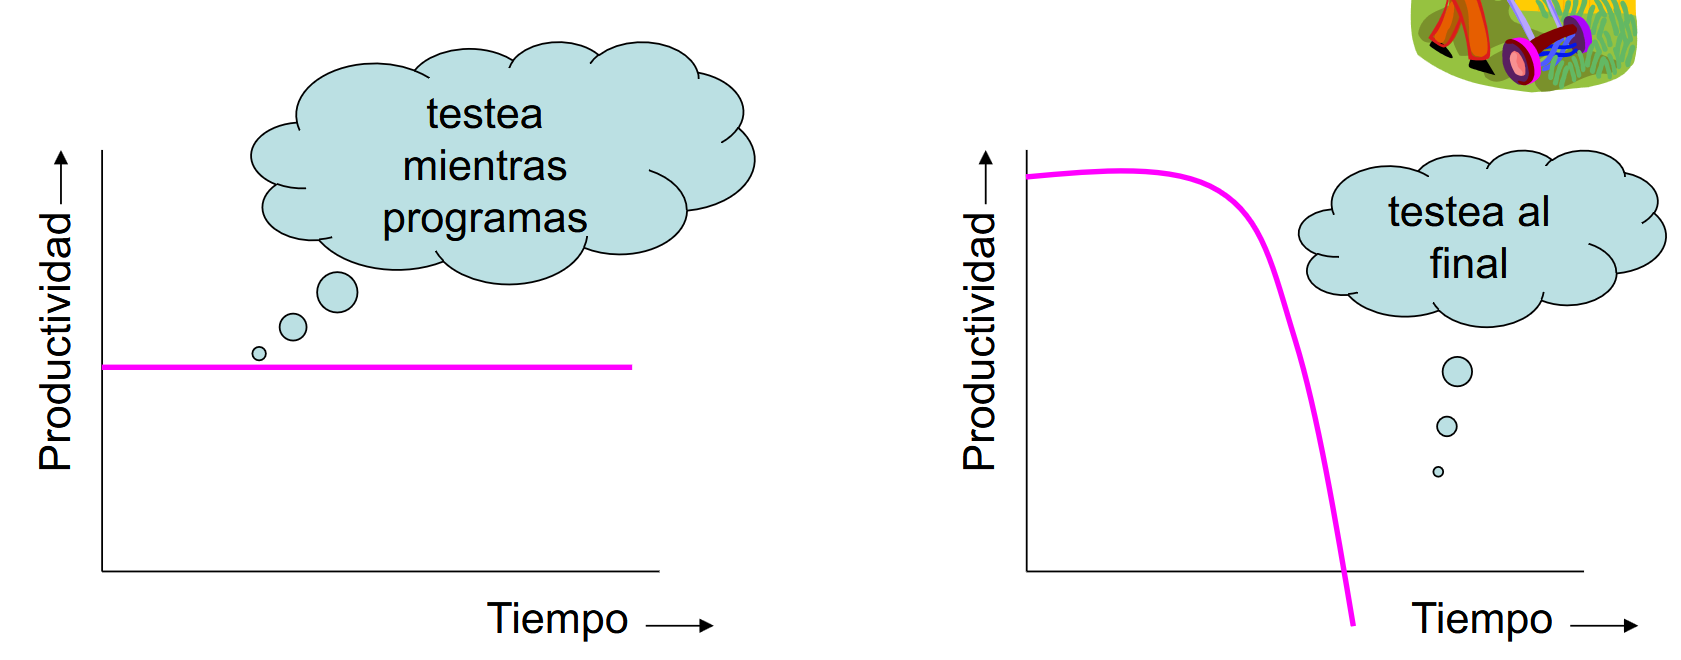
\includegraphics{images/03/unitPostpone.png}
   \caption{Posponer el testeo unitario cuesta mucho tiempo}
   \label{fig:03/unitPostpone}
\end{figure}

\coolquote{
   No es mi trabajo hacer testeo, tenemos un departamento de calidad
}{Bad programmer}

Entonces ¿cuál es el trabajo de un programador? El trabajo de cada programador es \ul{producir código que
funciona y que no contenga ``muchos'' errores}

\subsubsection{JUnit}

\begin{paracol}{2}
	
	\colfill
	JUnit es un framework de testing para Java. JUnit es una herramienta que ayuda a los programadores a escribir pruebas unitarias en Java. JUnit ha sido importante en el desarrollo de la metodología de programación extrema (XP).
	\lstinline|@Test| son los métodos de prueba.
	\begin{itemize}
		\item \lstinline|@BeforeEach| se invoca antes de la ejecución de cada test
		\item \lstinline|@AfterEach| se invoca después de la ejecución de cada test
		\item \lstinline|@BeforeAll| se invoca antes de la ejecución de todos los tests
		\item \lstinline|@AfterAll| se invoca después de la ejecución de todos los tests
	\end{itemize}
	
	\colfill
	\switchcolumn

	\begin{lstlisting}
public class TestDB {
	static private Connection dbConn;
	static private Account acc;
	@BeforeAll
	public static void setUpBeforeAll(){
		dbConn = new Connection("Oracle",15,fred, "f");
		dbConn.connect();
	}
	@AfterAll
	public static void tearDownAfterAll(){
		dbConn.disconnect();
		dbConn = null;
		}
	@BeforeEach
	protected void setUp(){
		acc = new Account();
		}
	@AfterEach
	protected void tearDown(){
		acc = null;
	}
	
	public void testAccountAccess(){
	.../Uses dbConn and acc
	}
	public void testEmployeeAccess(){
		.../Uses dbConn and acc
		}
\end{lstlisting}			
\end{paracol}

\begin{paracol}{2}
	
	\colfill
	En el ejemplo anterior, se muestra un test de una clase \texttt{Account} que tiene una conexión a una base de datos. Se puede ver que se crea una conexión a la base de datos en el método \texttt{setUpBeforeAll} y se cierra en el método \texttt{tearDownAfterAll}. Además, se crea una instancia de la clase \texttt{Account} en el método \texttt{setUp} y se destruye en el método \texttt{tearDown}.
	\colfill
	
	\switchcolumn
	Los metodos son ejecutados en el siguiente orden:
	\ns
	\begin{itemize}
		\item \lstinline|setUpBeforeAll|
		\item \lstinline|setUp|
		\item \lstinline|testAccountAccess|
		\item \lstinline|tearDown|
		\item \lstinline|setUp|
		\item \lstinline|testEmployeeAccess|
		\item \lstinline|tearDown|
		\item \lstinline|tearDownAfterAll|
	\end{itemize}
\end{paracol}

% TODO ejemplo factorial

\subsection{Testeo de Integración}

\begin{definition}
	[Testeo de Integración]
	El testing de las interfaces y la
	interacción entre las unidades previamente testeadas
	mientras que se ensambla el sistema entero
\end{definition}

\begin{itemize}
	\item ¿Qué componentes son el foco del testeo de integración?
	\item ¿En qué orden vamos a testear las interfaces?
	\item ¿Qué técnicas utilizamos para testear las interfaces?
\end{itemize}

Hay tres estrategias:
\begin{enumerate}
	\item \textbf{Big Bang} (todos los componentes a la vez)
	\item \textbf{Bottom-up} (de abajo hacia arriba)
	\item \textbf{Top-down} (de arriba hacia abajo)
\end{enumerate}

\begin{figure}[htbp]
	\centering
	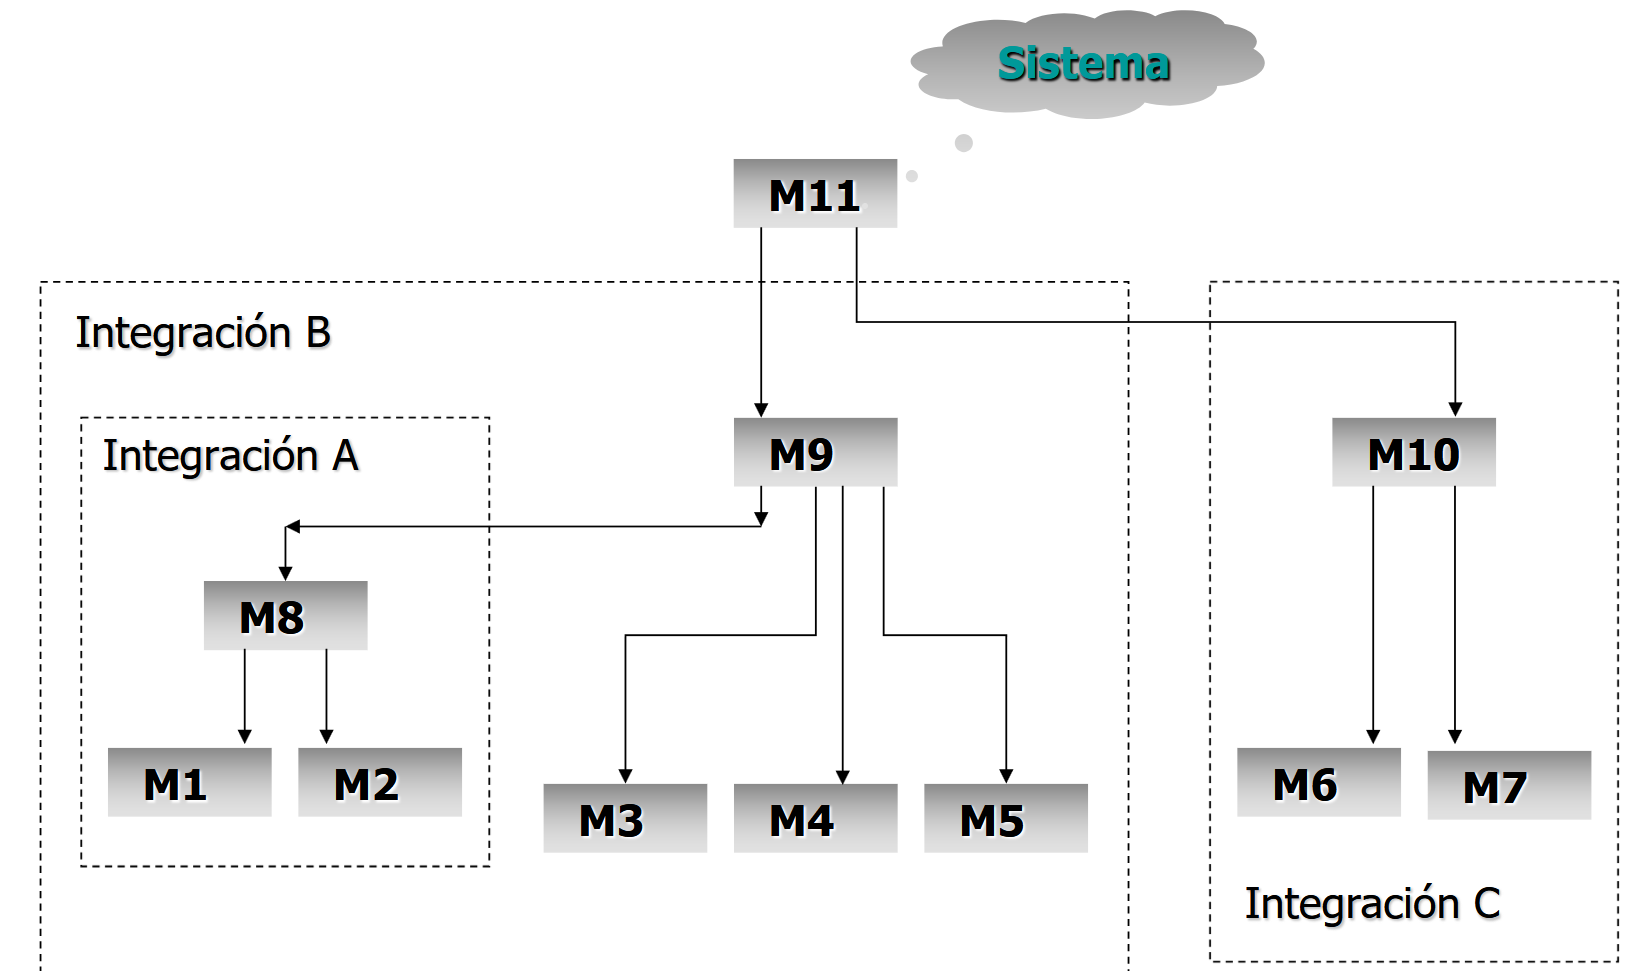
\includegraphics{images/03/bottomup.png}
	\caption{Arbol de dependencia y Bottom-up testing}
	\label{fig:03/bottomup}
\end{figure}

Para hacer el testing \textit{bottom-up} necesitamos \textbf{drivers}.
Un driver es un programa que invoca un componente bajo testeo, por ejemplo, para simular un componente de un nivel superior cuyo código todavía no está disponible (está todavía en desarrollo).

\begin{figure}[htbp]
	\centering
	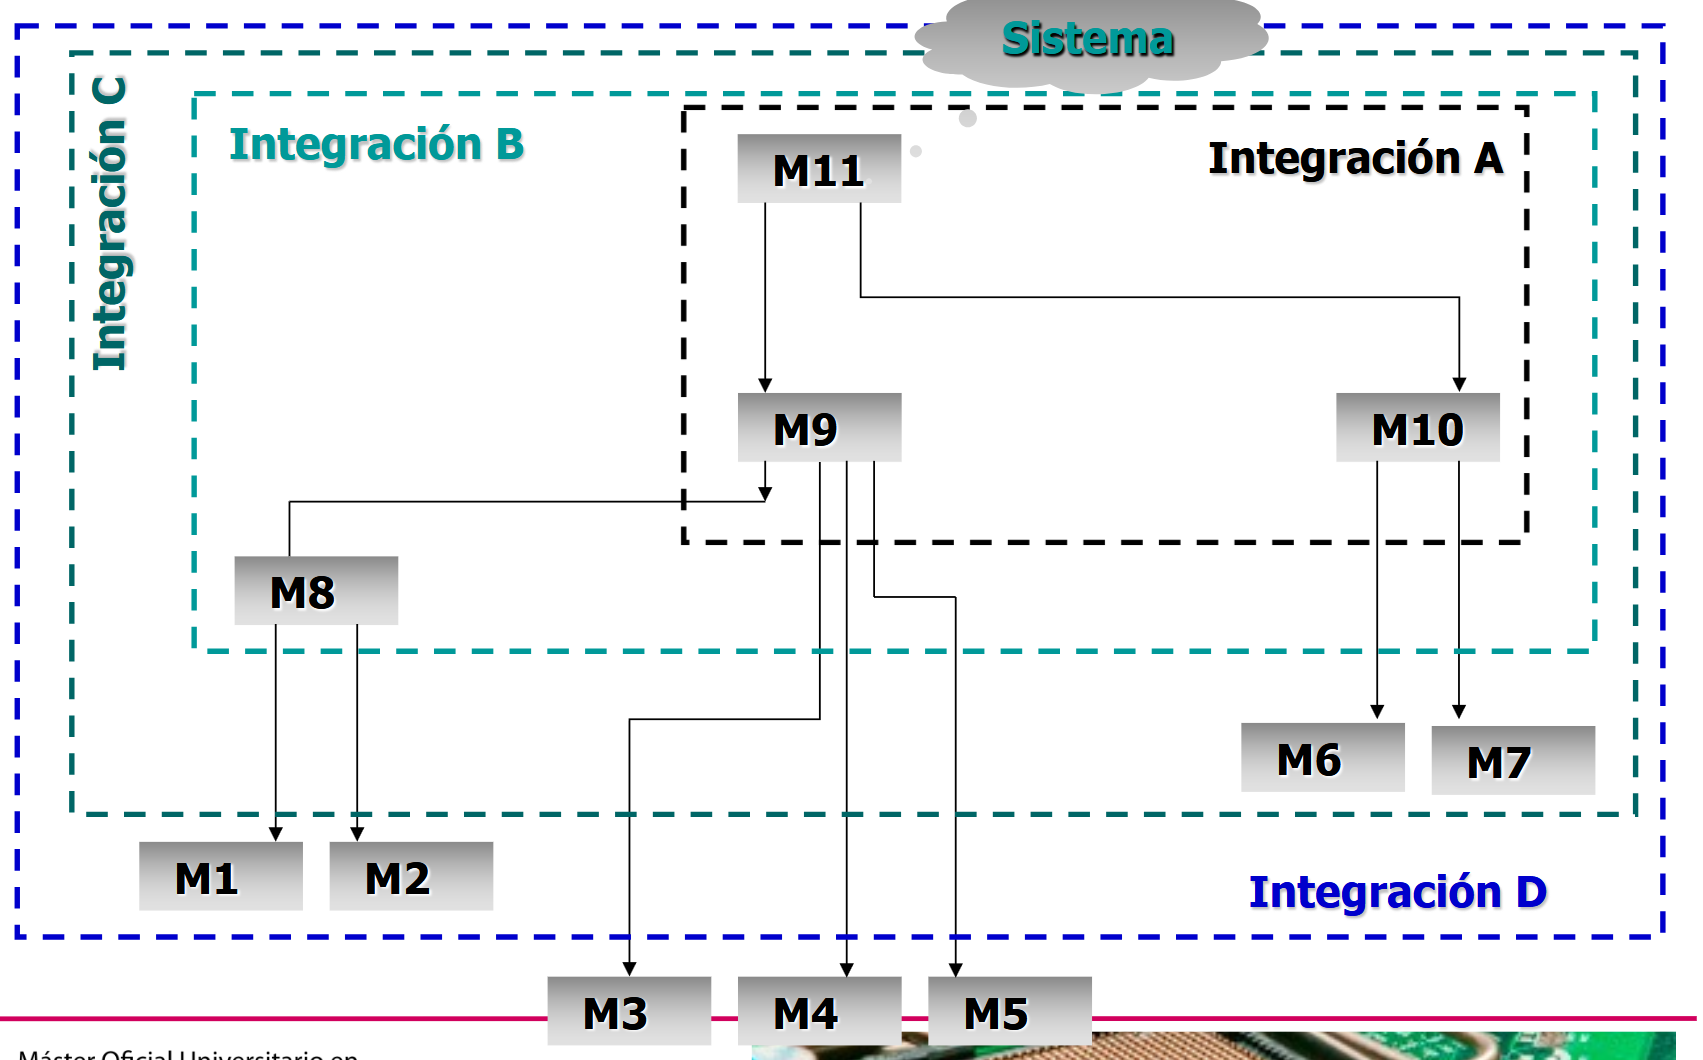
\includegraphics{images/03/topdown.png}
	\caption{Top-down testing}
	\label{fig:03/topdown}
\end{figure}

Para hacer el testeo de integración de manera \textit{top-down}, se
necesita dobles, que simulan componentes de un nivel inferior (``Stub'', ``dummy'', ``fake'', ``mock'').
\ns

El \textit{Big Bang} testing se utiliza solo para sistemas pequeños, ya que es muy difícil de manejar en sistemas grandes.


\subsubsection{Mockito}
Mockito es un framework de testing para Java que permite crear objetos simulados (mocks) de clases y interfaces. Mockito se utiliza para simular objetos que son necesarios para realizar pruebas unitarias. Se puede integrar con JUnit para realizar pruebas unitarias en Java. 
En las slides se muestran ejemplos de cómo utilizar Mockito.

Mockito es muy comodo para implementar el testeo de integración de manera \textit{top-down}.
% TODO Parte 2 y 3	

\section{Testeo de Sistema}
Se verifica que se cumple los requisitos especificados, es decir, que el sistema realiza correctamente todas las funcionesque se han detallado en las especificaciones dadas por el usuario del sistema.

Es necesario automatizar las prubas, y por esto se utilizan herramientas como \textit{Selenium}, que permite automatizar pruebas en navegadores web: en este caso, hablamos de pruebas de \textbf{funcionalidad}.

Para testar el \textbf{rendimiento} (tiempo de respuesta, carga, memoria.) se utilizan herramientas como \textit{JMeter} o \textit{NeoLoader}.

Otros aspectos importantes que el testeo debe cubrir son \textbf{Seguridad} y \textbf{Usabilidad}.

\section{Testeo de aceptación}
Esto testeo es dirigido a los criterios de aceptación
previamente establecidos con el cliente. Se puede hacer de manera manual o automatizada.

\subsection{Regresión}
Testeo que se necesita hacer después de cambios en el
software para asegurar que no se ha introducido defectos.

\ul{El testeo de \textbf{regresión} se tiene que automatizar} por el simple hecho de que el testeo de regresión manual \textit{NO SE HACE}.

\section{Gestión de Defectos, métricas y mas}

{El proceso de clasificación de defectos incluye tres fases:\ns
\begin{enumerate}
	\item Detección de defectos
	\item Investigación de defectos
	\item Resolución de defectos
\end{enumerate}}

\note{
\begin{itemize}
	\item \textbf{Actividad} (que estábamos haciendo cuando encontramos el fallo)
	\item \textbf{Fase del proyecto} (en que estábamos cuando encontramos el fallo)
	\item \textbf{Repetitividad} (¿se puede repetir el error?)
	\item \textbf{Síntoma} (fallo del sistema, mensaje de error, entrada no aceptado, resultado
incorrecto, etc.)
	\item \textbf{Causa} (nuestro producto, componente externo, usuario, etc.)
	\item \textbf{Origen} (especificación de requisitos, diseño, programación, etc.)
	\item \textbf{Impacto} (misión: crítico, medio, …; en la planificación; para el cliente, etc.)
\end{itemize}
}

\subsection{Métricas}


 Las métricas son observaciones cuantitativas para:
\begin{itemize}
	\item Informar sobre el \textbf{progreso del proyecto} de testeo
\note{\begin{itemize}
	\item ¿Qué tareas han terminado en tiempo?
	\item ¿Qué tareas han terminado antes?
	\item ¿Qué tareas han tenido retraso?
	\item ¿Cómo vamos siguiendo la planificación?
	\item Si no vamos bien, ¿cuáles son las razones?
	\item ¿Qué productividad ha tenido persona/equipo X?
\end{itemize}}
	\item Informar sobre la \textbf{calidad del software}
	\note{\begin{itemize}
		\item ¿Podemos parar el testeo?
	\item ¿Podemos entregar producto?
	\item ¿Hemos resueltos todos los defectos?
	\item ¿Cómo estamos gesHonando los defectos?
	\item ¿Cuántos defectos hemos encontrado por: subsistema,
	origen, causa, severidad, etc\dots?
	\end{itemize}}
	\item Informar sobre la \textbf{calidad del testeo}
	\note{\begin{itemize}
		\item ¿Estamos haciendo los tests necesarios?
		\item ¿Están siendo efectivos los tests?
		\item ¿Estamos utilizando los casos de prueba adecuados?
		\item ¿Necesitamos tener en cuenta diferentes casos de prueba?
	\end{itemize}}
\end{itemize}

La cobertura del testeo es una métrica importante para evaluar la calidad del testeo. La cobertura del testeo es la medida de la cantidad de código que ha sido ejecutado por los tests, especialmente en lo que se refiere a instrucciones, decisiones y condiciones (múltiples).\\
Pero puede referirse también a la cobertura de los requisitos, de los casos de uso, de los casos de prueba, etc.

\begin{lstlisting}[caption={Con 1 test donde \lstinline|x==y| se cubre todo el codigo, pero no todas las decisiones. En efecto, el defecto ocurre cuando \lstinline|x!=y|}]
	int foo_3 ( ) {
		int* p = NULL;
		int x;
		if (x==y) {
			p = &x;
		}
		*p = 123;
	}
\end{lstlisting}

\subsection{Mutación}

La mutación es una técnica de testing que consiste en introducir errores en el código fuente para ver si los tests son capaces de detectarlos. Se puede utilizar para evaluar la calidad de los tests.

\subsection{Organización del testing}
Se puede dedicar un equipo de testo integrado, con un jefe, o se puede haber que desarrolladores y testeadores son las mismas personas y no hay testeadores a tiempo completo.
La ventaja de tener un equipo de testeo es que se puede tener una visión más objetiva del software, ya que los testeadores no han desarrollado el software; al contrario, si los desarrolladores hacen el testeo, no tienen que comunicar con los testeadores, y conocen el software.

Otra tecnica de organización es \textit{Outsourcing}, que consiste en contratar una empresa externa para hacer el testeo. La ventaja es que se puede tener una visión más objetiva del software, y se puede tener acceso a expertos en testeo. La desventaja es que se puede tener problemas de comunicación, y que se puede tener problemas de confidencialidad.



\end{document}
